\subsection{Mapping Analysis Results to Classification Scheme} \textbf{Aim:} Analyze the collected data to identify recurring patterns and design a multi-level classification scheme for security faults. The goal is to move from raw data to insight, culminating in a hierarchical taxonomy (Dimension $\rightarrow$ Subclass $\rightarrow$ Example CWE) that reflects the observed diversity of vulnerabilities.
\newline

\textbf{Steps:}
\begin{itemize}
    \item \textbf{Exploratory Analysis.} We perform statistical and visual analyses on the dataset. This includes generating histograms of vulnerabilities by language, technology, and layer; heatmaps showing co-occurrence of attributes; and scatter plots for correlations (e.g. severity vs. time). These visuals help highlight the most prominent fault attributes and gaps.
    \item \textbf{Pattern extraction.} From the visualizations we identify recurring themes. For instance, we may observe that web-related vulnerabilities (CWE-79, CWE-89) cluster in the "Technology: Web" category, or that certain root causes (e.g. improper input validation, CWE-20) appear across multiple languages and frameworks.
    \item \textbf{Classification hierarchy design.} Guided by the unified attributes (from Phase I) and patterns, we construct a three-level classification. The top level ("Dimension") corresponds to our major analysis axes (e.g. {\em Programming Language}, {\em Technology Domain}, {\em Architectural Layer}, {\em Root Cause}). The second level ("Subclass") refines each dimension (e.g. for Language: {\em Web Languages} vs. {\em System Languages}). The third level lists concrete examples, typically specific CWE identifiers or vulnerability types (e.g. {\em CWE-79: XSS} under "Technology: Web"). An excerpt of this hierarchy is shown in Table~\ref{tab:classification}, and its conceptual organization is visualized in Figure~\ref{fig:classification-hierarchy}.
\end{itemize}

\begin{table}[h!]
\centering
\caption{Excerpt of the classification hierarchy (Phase III): Dimension $\rightarrow$ Subclass $\rightarrow$ Example CWE.}
\label{tab:classification}
\begin{tabular}{lll}
\hline
\textbf{Dimension} & \textbf{Subclass} & \textbf{Example CWE} \\
\hline
Language & Web-facing languages & CWE-79 (Cross-site scripting) \\
Language & System languages & CWE-120 (Buffer overflow) \\
Technology & Web frameworks & CWE-89 (SQL injection) \\
Technology & Mobile applications & CWE-22 (Path traversal) \\
Layer & Network layer & CWE-319 (Cleartext transfer) \\
Layer & Application layer & CWE-416 (Use-after-free) \\
Root Cause & Input validation errors & CWE-20 (Improper input check) \\
Root Cause & Memory management errors & CWE-119 (Buffer overflow) \\
\hline
\end{tabular}
\end{table}


\begin{figure}[!h]
	\centering
    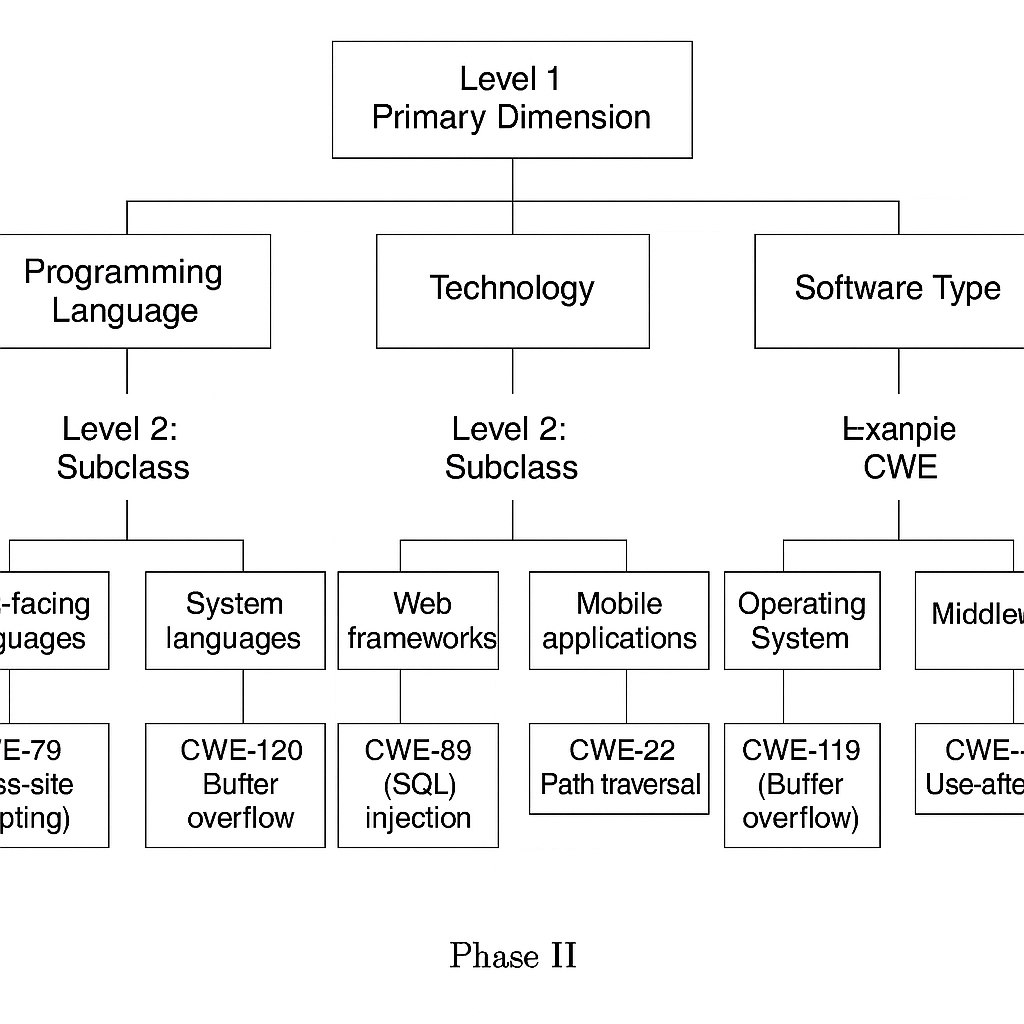
\includegraphics[width=0.55\textwidth]{figures/chapter_2/classification-hierarchy.png}
	\caption{Hierarchical classification}
	\label{fig:classification-hierarchy}
\end{figure}


Figure~\ref{fig:classification-hierarchy} (above) sketches the hierarchical classification derived in Phase III. Each Dimension branches into subclasses with illustrative CWE examples at the leaves. This taxonomy is rooted in the empirical data patterns uncovered and in prior taxonomies cited earlier. Through these steps, Phase III links the aggregated data back to our taxonomy framework, revealing how software vulnerabilities distribute across the multi-dimensional space. The resulting classification scheme provides a structured way to profile security faults, based both on existing knowledge (the taxonomies) and new insights from the data analysis.